% Chapter Template

\chapter{Grundlagen} % Main chapter title

\label{Kaptiel3} % Change X to a consecutive number; for referencing this chapter elsewhere, use \ref{ChapterX}

%----------------------------------------------------------------------------------------
%	SECTION 1
%----------------------------------------------------------------------------------------
\section{Graph}

Ein Graph ist eine abstrakte Datenstruktur, welche für die GDBs verwendet werden \parencite{vicknair2010comparison}. Ein Graph besteht aus einer endlichen nicht leeren Summe von Knoten, auch Vertex oder Punkte genannt und Kanten. Die Kanten des Graphen bildet die Verbindung zwischen zwei Knoten \url{ http://wwwmayr.in.tum.de/lehre/2008WS/ea/EA-7.pdf}(7.06.19), wenn die Kanten aus einem geordneten Paar bestehen und somit eine Richtung besitzen wird der Graph als gerichtet bezeichnet, bei einem ungeordneten Paar wird von einem ungerichteten Graph gesprochen\parencite{bondy1976graph}. Wenn die Kanten Attribute, wie zum Beispiel Kosten besitzen wird der Graph als gewichtet bezeichnet und ohne Attribute als ungewichtet  \url{ http://wwwmayr.in.tum.de/lehre/2008WS/ea/EA-7.pdf}(7.06.19). 

%-----------------------------------
%	SUBSECTION 1
%-----------------------------------
\section{Neo4j}

Neo4j ist eine Graphdatenbank, welche in Java implementiert wurde \parencite{vukotic2015neo4j}. Als Grundlegende Datenstruktur wird ein gerichteter und gewichteter  Graph verwendet.Knoten stellen die Entitäten,beispielsweise eine Person oder ein Produkt,  da und  Kanten stellen die Relationen zwischen den Entitäten da, beispielsweise “isAngestellt” und können optional ein Gewicht und eine Richtung besitzen. Attribute können als zusätzliche Informationen in den Knoten gespeichert  werden wie zum Beispiel: Name bei einem Knoten “Person”. Knoten können mit Bezeichnern versehen werden, um so leichter in Anfragen  verwendet werden zu können. Die Operationen sind entweder durch durch die  Anfragesprache  Cypher,welche eine standardisierten Syntax mit  mehreren vordefinierten Funktionen besitzt, limitiert oder durch die jeweilige verwendete Programmiersprache.Es wird das Einbetten weiterer Bibliotheken, welche weitere Funktionen oder Algorithmen stellen, unterstützt. Durch weitere Funktionen wie zum Beispiel die Bibliothek “APOC” \footnote{https://neo4j-contrib.github.io/neo4j-apoc-procedures/ (17.05.19) } ist es möglich, Daten aus verschiedenen Formaten wie JSON,XSL oder XML in die Datenbank zu laden oder Daten aus anderen Web-APIs zu nutzen. Neo4j lässt sich in einem  eingebetteten Modus oder einem  Server Modus nutzen. Der eingebettete Modus dient der direkten  Nutzung durch die Java Core API(Application programming interface)  von Neo4j. Der Server Modus ermöglicht eine getrennte Ausführung von dem Code und dem bestehenden Neo4j System.

\section{Neo4j als Datenbank management system}
Ein Datenbank Managment System(DBMS), ist für die Verarbeitung von Anfragen verantwortlich und kann mit folgenden Teilen beschrieben werden: Eine Schnittstelle mit dem Nutzer, eine Anfragesprache, ein Anfrage-Optimierer, eine storage engine ,eine transaction engine, eine database engine und operation features, zum Wiederherstellen von Daten \parencite{angles2012comparison}. Als Schnittstelle mit dem Nutzer stehen die Anwendungen “Neo4j Browser” unter Linux und “Neo4j Desktop” unter Windows zur Verfügung, zusätzlich besteht die Möglichkeit eine von den Neo4j Treibern unterstützte Programmiersprache  oder Java zu verwenden und direkt die Neo4j APIs zu nutzen. Die Anfragesprache für Neo4j Browser und Neo4j Desktop ist “Cypher”. Zum Optimieren von Anfrageplänen wird der “Cypher Query Optimizer”verwendet. Die wird storage engine durch die Record Files und die transaction unit  wird durch das Transaction Management dargestellt. Die database engine bildet das Gesamtsystem der einzelnen Komponenten. Die operation features zum Wiederherstellen von Daten werden in dem Transaktions-Log realisiert. Optional kann zu eventuellen Performanz Steigerung ein Cache verwaltet werden. In der Neo4j Enterprise Version ist es möglich, das DBMS auf mehrere Systeme in einem Netzwerk mittels High Availability Funktion auszulagern \parencite{vukotic2015neo4j}. Zusammengefasst wird die Architektur in \ref{fig:Architecure}

\begin{figure}[th]
	\centering
	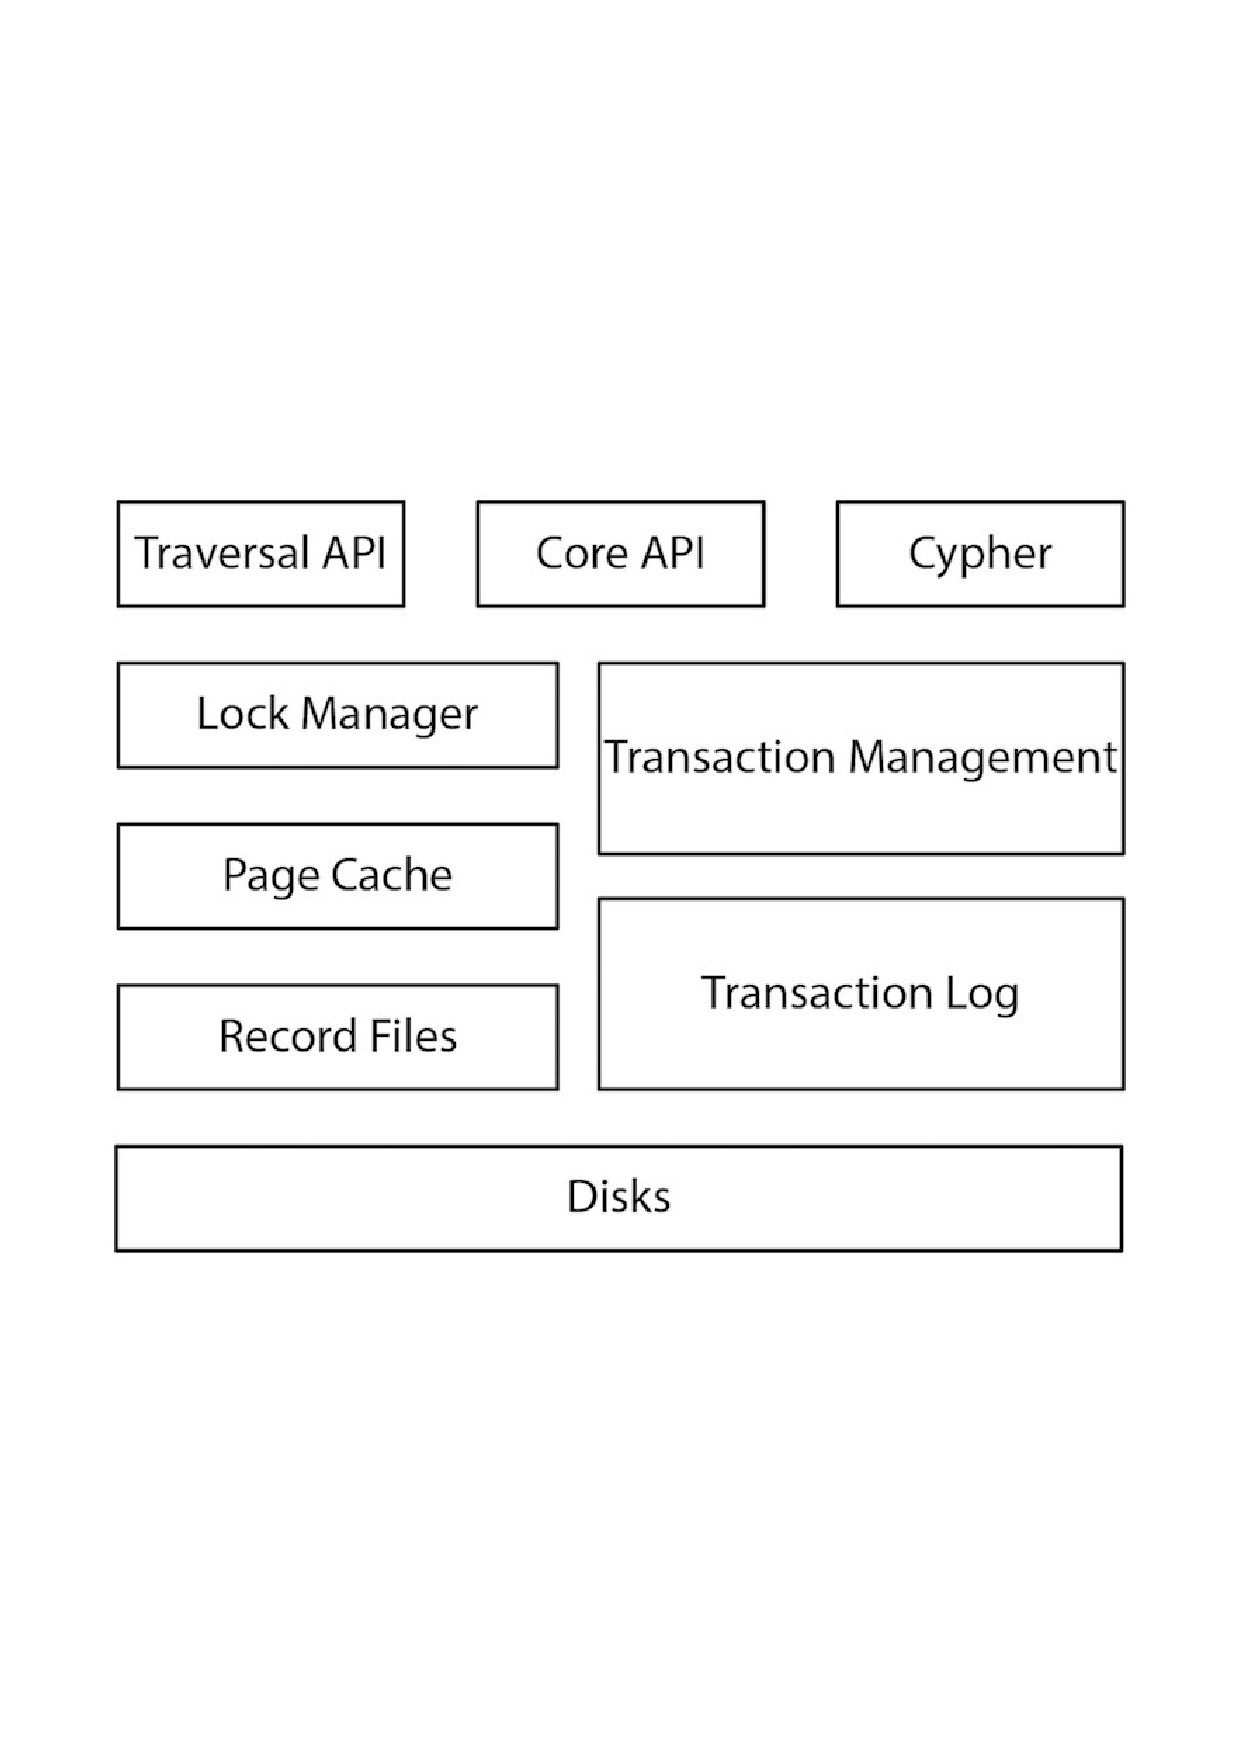
\includegraphics [width=13cm, height=14cm]{Figures/Architecure}
	\caption[Architecture]{Allgemeine Architektur von Neo4j.}
	\label{fig:Architecure}
\end{figure}

\subsection{Cypher und APIs für Neo4j}
Im Folgenden werden die Möglichkeiten zum Interagieren mit Neo4j beschrieben. Da es über die Neo4j-Treiber möglich ist, Neo4j in mehreren Programmiersprachen zu nutzen und die genaue Anzahl der Sprachen stetig steigt, werden im folgenden nur die Kernfunktionen in Java beschrieben und verwendet. Im späteren Absatz zu Neo4j im Servermodus wird zusätzlich das Bolt-protocol und die REST HTTP API beschrieben, welche als weitere Schnittstelle dienen.

\subsubsection{Cypher}
Im Gegensatz zu den relationalen Datenbanken gibt es bei Graphdatenbanken keine standardisierte Anfragesprache, welche bei den meisten Graphdatenbanken Verwendung findet \parencite{han2011survey}. In Neo4j besteht seit 2000 die Möglichkeit die deklarative Anfragesprache “Cypher” zu verwendenden  \parencite{francis2018cypher}. Cypher wird von Neo4, Inc. entwickelt und wurde ursprünglich ausschließlich für die Neo4j Datenbank verwendet. Seit Oktober 2015  findet Cypher als “openCypher” Gebrauch in anderen Datenbanken \parencite{francis2018cypher}. Da für die Traversal API und die Java Core API Kenntnisse in Java bzw. einer durch die Neo4j-Treiber unterstützten Programmiersprachen benötigt werden, bildet Cypher eine Möglichkeit ohne diese Kenntnisse mit der Datenbank zu interagieren[16]. Die Syntax ist an SQL und Gremlin \parencite{vukotic2015neo4j} orientiert. In Cypher wird ein Muster von dem Nutzer angegeben und alle Objekte, die dieses Muster erfüllen, können zurückgegeben werden. Die wichtigsten  Schlüsselwörter sind: \newline
\textbf{Where}: Dies hat die gleiche Funktion wie in SQL und spezifiziert Objekte durch einen Ausdruck. \newline
\textbf{Match}: Dadurch wird das Muster spezifiziert indem Neo4j suchen soll. Beispielweise: 
\begin{Verbatim}[frame=single]
MATCH (p1:Person)-[:Friends]->(p2:Person) 
WHERE p1.name= ‘Peter’ 
RETURN p.name
\end{Verbatim}
, hier werden alle Personen-Knoten durchsucht, die mit einer “Friends”-Relation mit dem Personen-Knoten von “Peter” verbunden sind. p1 stellt ein Label für den Knoten vom Typ “Person” da, [:Friends] ist eine Relation vom Typ “Friends” und durch “->” wird angegeben, dass es sich um eine ausgehende Kante vom Knoten p1 handelt. \newline
\textbf{Return}: Es wird angegeben, welche Objekte bzw. welche Attribute der Objekte, die das Muster erfüllen zurückgegeben werden sollen.\newline
\textbf{Delete}: Wie in SQL  wird ein Objekt  oder mehrere Objekte aus der Datenbank entfernt.\newline
\textbf{With}: Dadurch lassen sich in einer Anfrage Objekte manipulieren bevor sie zu einer weiteren Anfrage gegeben werden. Beispielsweise:
\begin{Verbatim}[frame=single]
MATCH (p:Person{name: ‘Peter’})  
WITH COUNT(p) as count  
RETURN count
\end{Verbatim} 
\textbf{Create}: Erzeugt ein Objekt in der Datenbank Beispielsweise 
\begin{Verbatim}[frame=single]
Create (p:Person)
\end{Verbatim}
, hier wird ein Knoten vom Typ Person erzeugt. Es ist auch möglich mehrere Knoten mit den dazugehörigen Relationen zu erzeugen. Indizes  für die Objekte oder Attribute von Objekten können ebenfalls über Create erzeugt werden.\newline
\textbf{Limit}: Beschränkt die Menge, welche durch das Return-Statement zurückgegeben wird Beispielsweise
\begin{Verbatim}[frame=single]
MATCH (p:person) RETURN p.name LIMIT 10
\end{Verbatim} 
, hier werden nur die Namen  von 10 Personen zurückgegeben\newline
\textbf{SUM/COUNT/AVG}: Werden wie in SQL verwendet. \newline
Der Nutzer beeinflusst so welche Daten durch  das Musters gesucht werden. Der Nutzer besitzt keine Möglichkeit die Art der Berechnung zu beeinflussen. Cypher wird dadurch als Nutzerfreundlichere, aber auch weniger performante Alternative zu den APIs empfohlen \parencite{vukotic2015neo4j}. In den folgenden Experimenten wurde sowohl Cypher als als auch die Travese API für einen direkten Vergleich verwendet. Cypher lässt sich ausschließlich als single thread ausführen.

\subsubsection{Java Core API}
Als low-level Schnittstelle zu den Kernfunktionen von Neo4j ist dies die Möglichkeit mit der besten Laufzeit \parencite{vukotic2015neo4j}. Zur Verwendung dieser imperativen API sind weitreichende Programmierkenntnisse und Wissen über die Neo4j-Bibliotheken, sowie einer genauen Vorstellung über die Daten in dem Graph erforderlich. Wenn diese Kenntnisse gegeben sind, ist die API sehr flexible verwendbar  und der Nutzer hat hohen Einfluss darauf, wie die Anfragen bearbeitet werden sollen und kann so eine optimale Berechnungsstrategie angeben \parencite{vukotic2015neo4j}. Die so produzierten Queries sind in meisten sehr lang. Eine Beispielhafte Berechung wäre:
\begin{Verbatim}[frame=single]
try ( Transaction tx = graphDb.beginTx() )
{
	Node Peter = graphDb.getNodeById(Peter_ID);
	Set<Node> friends = new HashSet<Node>();
	for (Relationship R : Peter.getRelationships(FRIEND)) {  
		Node friend = R.getOtherNode(userJohn);
		friends.add(friend);                        
	}
	for (Node friend : friends) {
	  logger.info("Found friend: " + friend.getProperty("name")); 
}

\end{Verbatim}
Bei diesem Beispiel werden alle Freunde von Peter gefunden und zurückgegeben.Der Nutzer gibt jede Transaktion explizit an,so ist es dem System möglich alle zur Verfügung stehenden Kerne zu nutzen.

\subsubsection{Traversal API}
Diese deklarative API  dient zum spezifizieren von Traversierungen im Graph, sie ist schneller als Cypher und langsamer als die Core API. Die Traversal API erlaubt einen high-level Zugriff auf Neo4j, welcher weniger abstrakt als die Core API ist und dennoch Programmierkenntnisse erfordert. Der Nutzer muss keine genaue Vorstellung von den Daten im Graphen haben.Es wird eine Beschreibung angegeben, wie eine Suche  genau ausgeübt werden soll und kann diese dann auf einen Knoten anwenden. 
\begin{Verbatim}[frame=single]
private Traverser getFriends(final Node person)
{
TraversalDescription td = graphDb.traversalDescription()
.relationships( RelTypes.FRIEND, OUTGOING )
.evaluator( Evaluators.atDepth(2) );
return td.traverse( person );
}
\end{Verbatim}
Zusammengefasst wäre diese Traversierung: Suche alle Verbindungen von dem Anfangsnode über die Relation FRIEND bis zu Tiefe 2.  Beim Traversieren kann der der Nutzer zwischen 2 grundsätzlichen Vorgehen wählen: Breadth-first und Depth-first, diese haben abhängig von der Struktur des Graphen eine unterschiedliche Laufzeit \parencite{vukotic2015neo4j}. \newline
\textbf {Breadth-First(Breiten-Suche)} : Zuerst werden alle Knoten mit derselben Distanz betrachtet, danach werden alle Knoten mit der nächst höheren Distanz betrachtet, dies wird solange ausgeübt bis alle Knoten betrachtet wurden. \newline
\textbf {Depth-First(Tiefen-Suche)} : Zuerst wird ein Nachbarknoten mit der geringsten Distanz betrachtet, ausgehend von diesem Nachbarknoten werden alle Nachbarn betrachtet. Wenn alle Nachbarn betrachtet wurden, wird ausgehend von Anfangsknoten ein weiterer Nachbar mit der geringsten oder nächst-geringsten Distanz untersucht und ausgehend von diesem werden erneut alle Nachbarn angeschaut. Dieses Vorgehen wird als Normalfall angenommen, wenn keine Vorgehen von dem Nutzer angegeben wird, wird dieses verwendet. 
\newline
\newline
Wenn der Nutzer mit der Struktur der Daten in dem Graph vertraut ist, kann das ausgewählte eine erheblichen Performance Unterschied  hervorbringen[16]. Die Traversion kann auch bidirektional aufgeführt werden, dabei werden 2 Anfangsknoten angeben und die Suche wird so lange ausgeführt, bis es zu einer Kollision der beiden Knoten kommt. Wenn eine Kollision zwischen den beiden Knoten erkannt wird, ist damit zum Beispiel eine Verbindung der beiden Knoten bewiesen. Für die folgenden Experimente wurde bei den meisten Anfragen die Traversal API verwendet. 

\subsection{Anfragebearbeitung und Planoptimierung}
Nach Angaben von Neo4j\footnote{https://neo4j.com/blog/introducing-new-cypher-query-optimizer/  (11.06.19)}, werden Anfragen, die mittels Cypher gestellt werden, nach folgendem Muster bearbeitet:
\begin{enumerate}
	\item Umwandeln der Eingabe in einen Abstrakten Syntax Baum (ASB)
	\item Optimieren des ASB
	\item Erstellen eines Anfrage Graphen aus dem Baum
	\item Erstelle einen logischen Plan
	\item Schreibe den logischen Plan neu
	\item Erstelle einen Ausführungsplan aus dem logischen Plan
	\item Führe die Anfrage mit Hilfe, des Ausführungsplans aus 
\end{enumerate}
Die Schritte 2-5 werden vom Anfrage-Optimierer übernommen. \newline
\newline
2. Die Optimierung des AST beinhaltet folgende Schritte: 
\begin{enumerate}
	\item Alle Labels, die sich in einem \textbf{Match} befinden, werden in das \textbf{Where}-Prädikat verschoben
	\item  Semantisch-Äquivalente \textbf{Where}-Prädikate werden zusammengefasst
	\item Ersetze alle Synonyme zum Beispiel: \textbf{RETURN * => RETURN x as x, y as y}
	\item Fasse Konstanten zusammen zum Beispiel: \textbf{3 + 3 => 6}
	\item Setze bei anonymen Knoten einen Namen ein zum Beispiel: \textbf{ MATCH () => MATCH (n)}
	\item Ersetze das Gleichheitszeichen durch ein 'IN'wie: \textbf{MATCH (n) WHERE id(n) = 12 => MATCH n WHERE id(n) IN [12]}
\end{enumerate}
3. Durch das erstellen einen Anfragegraphen, wird ein abstraktere high-level Darstellung für die Anfrage erzeugt. Diese lässt sich kosteneffizienter Optimieren.	 \newline \newline
4. Aus dem Anfragegraph werden logische Pläne für jede Anfrage erzeugt. Dieser Plan ist ein Baum mit maximal 2 Kindern, welche die verwendeten Operatoren darstellen. Dies gleicht dem logischen Plan für relationnelle Datenbanken. Aus dem logische Plan wird der geschätzte Bearbeitungsaufwand für eine Anfrage gelesen. Der Aufwand wird aus den benötigten I/O-Operatoren auf den Speicher oder Indizies und den durchzuführenden Traversierungen ermittelt. Bei jedem Durchgang werden mehrere Pläne für eine Anfrage erzeugt, der Optimierers wählt aus diesem Plänen mit einem gierigen Suchalgorithmus einen Plan aus, welcher nicht immer der optimalste Plan ist. Der gierige Suchalgorithmus gewährleistest, dass nicht der langsamste Plan gewählt wird, aber es ist nicht garantiert, dass der optimalste Plan gewählt ist. \newline \newline
5. Nachdem die Pläne erstellt wurden und einer dieser Pläne ausgewählt wurde, wird der ausgewählte Plan nochmals optimiert. Das heißt mehrere Komponenten werden vereinfacht oder zusammengeführt und jede Art von Verschachtelung wird aufgelöst. \newline \newline
Nach diesem Schritt  ist die Arbeit des Optimierers abgeschlossen und die Database-Engine kann aus diesem optimierten Plan einen ausführbaren Plan erstellen. 

\subsection{Speicherverwaltung in Neo4j}
Graphdatenbanken besitzen eine andere Speicherverwaltung als relationnelle Datenbanken \parencite{angles2012comparison}. In Neo4j wird der Speicher in sogenannten Record Files unterteilt, diese Dateien speichern jeweils einen Teil des Graphen ab, wie Knoten, Kanten, Eigenschaften etc.. Die Objekte besitzen in den Dateien eine feste Größe, dies erlaubt einen Zugriff in O(1) \parencite{robinson2013graph}. Wenn zum Beispiel der Knoten mit der ID "100" gesucht wird und ein einzelner Knoten X Bytes groß ist, wird der gesuchte Knoten bei Byte 100*X beginnen. Die genaue Größe  variiert, je nach betrachteter Neo4j Version, seit Neo4j Version 3.X besitzt ein Knoten die Größe 15 Byte und werden in node-store gespeichert. \footnote{https://neo4j.com/developer/kb/understanding-data-on-disk/ (13.06.19)}. Nach \parencite{robinson2013graph} werden die Objekte wie folgt verwaltet:
\subsubsection{Verwaltung der Knoten im Speicher}
Ein Knoten im Knotenspeicher wird folgendermaßen dargestellt: Das erste Byte kennzeichnet, ob der Knoten verwendet wird bzw. verwendet werden kann. Die nachfolgenden 4 Bytes kennzeichnen die ID für die erste Relation, die mit dem Knoten verbunden ist. Die darauffolgenden 4 Bytes beschreiben das erste Attribute des Knoten. Die nächsten 5 Bytes verweisen auf ein Label, welches gegebenenfalls verwendet wurde und ich sich im Label-Store befindet. Das Letzte Byte ist für bestimmte Flags und für zukünftige Arbeiten. 
\subsubsection{Verwaltung der Kanten im Speicher}
Die Kanten werden in dem Relationsspeicher gespeichert. Jeder Eintrag besitzt die IDs zu den zugehörigen Knoten, einen Pointer zu dem Relationstypen, welcher in dem Relationstypspeicher gespeichert ist, Pointer zu den vorherigen und nächsten Relationen von den beiden zugehörigen Knoten und ein Flag das angibt, ob die betrachtete Relation die erste ist. \newline
\subsubsection{Verwaltung der Eigenschaften im Speicher}
Da Neo4j eine property graph databse ist, kann jeder Knoten und jede Kante  Eigenschaften besitzen. Die Eigenschaften befinden sich im Eigenschaftenspeicher.  Jeder Eintrag zu einer Eigenschaft ist in 1-4 Blöcke und eine ID zu einer folgenden Eigenschaft unterteilt. Jeder dieser Blöcke beinhaltet Informationen über einen Typen, welcher ein standard- Java-Typ, string oder ein Array sein kann und Informationen über einen Pointer auf einen Index, der auf den Namen der Eigenschaft verweist, zeigt.  \newline
\subsubsection {Traversierung im Speicher}
Die festgelegte Größe der Knoten und Kanten hat als Ziel die Traversierung zu beschleunigen \parencite{robinson2013graph}. Eine einfache Traversierung wird beschrieben wie folgt: 
\begin{enumerate}
	\item Starten bei einem Eintrag in den Knotenspeicher
	\item Lesen des gegebene Byte für die ID zur ersten Relation und betrachten des entsprechenden Eintrags im Relationsspeicher mit dieser ID
	\item Ausgehend von dem Eintrag im Relationsspeicher wird der Pointer zum dazugehörigen Knoten aufgerufen.
	\item Springen zu der Knoten im Knotenspeicher
\end{enumerate}
Diese Traversierung beschreibt das suchen eines benachbarten Knotens.
\subsubsection{Caching im Speicher}
LRU-K page-affined cache beschreibt, dass der Speicher aufgeteilt wird und eine feste Anzahl von Teilen wird im Speicher gehalten. Die Auswahl, der Teile die im Speicher gehalten werden geschieht nach der least frequently used(LFU) Methode. Die Methode besagt, dass ein Teil der selten benutzt wird aus dem Speicher entfernt wird und ein häufig genutzter Teil wird in dem Speicher gehalten \parencite{robinson2013graph}.
\subsection{CAP und ACID unter Neo4j}
Das CAP-Theorem charakterisiert  das Verhalten einer Datenbank anhand von folgenden 3 Eigenschaften: Consistency(Konsistenz), Availability(Verfügbarkeit), Partitionstoleranz \parencite{simon2000brewer}. Konsistenz beschreibt die Eigenschaft, dass die Daten in allen Partitionen zur selben Zeit dieselben Werte besitzen und das gleiche Verhalten aufweisen. Verfügbarkeit beschreibt die Möglichkeit zu jeder Zeit eine Anfrage an das System stellen zu können und auch zu jeder Zeit eine Antwort auf die gestellte Anfragen bekommen zu können. Partitionstoleranz gewährleistet, dass sich das Verhalten des System nicht verändert, wenn mehrere Partitionen von diesem System erstellt werden und alle Partitionen müssen das gleiche Verhalten aufweisen  \parencite{simon2000brewer}. Neo4j erfüllt die Bedingung der Verfügbarkeit und der  Partitionstoleranz[16] und wird so als “AP-Database” bezeichnet. \newline
Die ACID Eigenschaft setzt sich aus 4 Eigenschaften zusammen, die das Verhalten der Transaktionen einer  Datenbank beschreiben \parencite{haerder1983principles}. Atomicy(Atomisch) beschreibt, dass jede Transaktion einzeln betrachtet wird und nur fehlschlagen oder erfolgreich sein kann. Durch Consistency(Konsistenz) kann jede Transaktion nur valide Daten verwenden und den validen Zustand einer Datenbank nicht in einen nicht-validen Zustand überführen. Isolation erwartet, dass jede Transaktion unabhängig von einer parallel-laufenden Transaktion abläuft und keine dieser Transaktionen beeinflusst. Durability(Haltbarkeit) ist gegeben, wenn der Effekt einer Transaktion auf den Speicher ausgeübt wurde und auch bei einem Absturz des Systems beibehalten wird \parencite{haerder1983principles}. Solange Neo4j auf einem einzelnen System läuft und nicht das High Aviability Feature der Enterprise Edition nutzt, ist es ACID konform \parencite{holzschuher2013performance}. Das atomische und haltbare Verhalten wird durch das sogenannte write-ahead log(wat) versichert. Bei diesem Mechanismus  werden alle Operationen einer Transaktionen nach dem Beenden der Transaktion in einem Log-File  festgehalten, bevor diese  den Speicher beeinflussen, so kann auch bei einem Absturz des System das Log-File genutzt werden um ein vorherige Transaktion zu wiederholen.  Dieses Log-File wird auch für die High-Availability  genutzt, welche es erlaubt die Datenbank in einem Netzwerk auf mehrere Systeme zu verwenden, dennoch ist es nicht mehr möglich ein  ACID Verhalten zu gewährleisten, da keine absolute Garantie für ein  atomisches und konsistente Verhalten gibt \parencite{vukotic2015neo4j}. Eine weitere versicherung für das atomische Verhalten bildet das Verhindern von Deadlocks innerhalb der Transaktion. Zur Verhinderung von Deadlocks wird “RWLock” verwendet, was eine Implementierung des Java “ReentrantReadWriteLock” für Neo4j ist. Dieser verwaltet alle Schreibsperren, die während einer Transaktion erstellt werden und versucht potentielle Deadlocks zu erkennen \parencite{raj2015neo4j}.
\section {Modi in Neo4j}
Wenn der Nutzer Neo4j nicht über die Anwendungen "Neo4j Browser/Desktop" nutzen möchte sonder über ein Programmiersprache  lässt sich Neo4j in 2 Modi nutzen, den eingebetteten Modus und den Server Modus. Diese Modi geben an wie die Bibliotheken von Neo4j, welche für die Anfragen des Nutzer benötigt werden, aufgerufen und verwendet werden. Dafür wird das Verhalten der Java Viral Machine (JVM), welche die Kompatibilität des geschriebenen Java-Codes gewährleistet, angepasst. Der verwendete Speicher ist für bei Modi der selbe.

\subsection{Der eingebettete Modus}
Der eingebettete Modus erlaubt es dem Nutzer mittels jeder Programmiersprache, die von der JVM unterstützt wird und für die ein Treiber zur Verfügung steht, die Bibliotheken von Neo4j zu nutzen und so Anfragen an den Datenbank zu stellen. Alle Bibliotheken von Neo4j werden von dem GraphDataBaseService von Neo4j verwaltet. Dieser Modus wird für die meisten Anwendungen, die auf einem einzelnen System laufen, empfohlen \parencite{raj2015neo4j}. Dies ist damit begründet, dass das Gesamtsystem im einbetteten Modus schneller läuft als im Server Modus, aber auch nur auf einem System genutzt werden kann, da sowohl alle Neo4j Funktionen als auch die Anfragen in der selben JVM agieren. Der Nutzer hat so volle und alleinige Kontrolle über jede Transaktion und kann jede zur Verfügung stehenden  API nutzen. Daraus resultiert, dass er Nutzer für ein sicheres starten und beenden der Datenbank in seinem Anfragecode verantwortlich ist\parencite{robinson2013graph}.  Verdeutlicht wird dieses Verhalten in \ref{fig:Embedded}.
\begin{figure}[!htb]
	\centering
	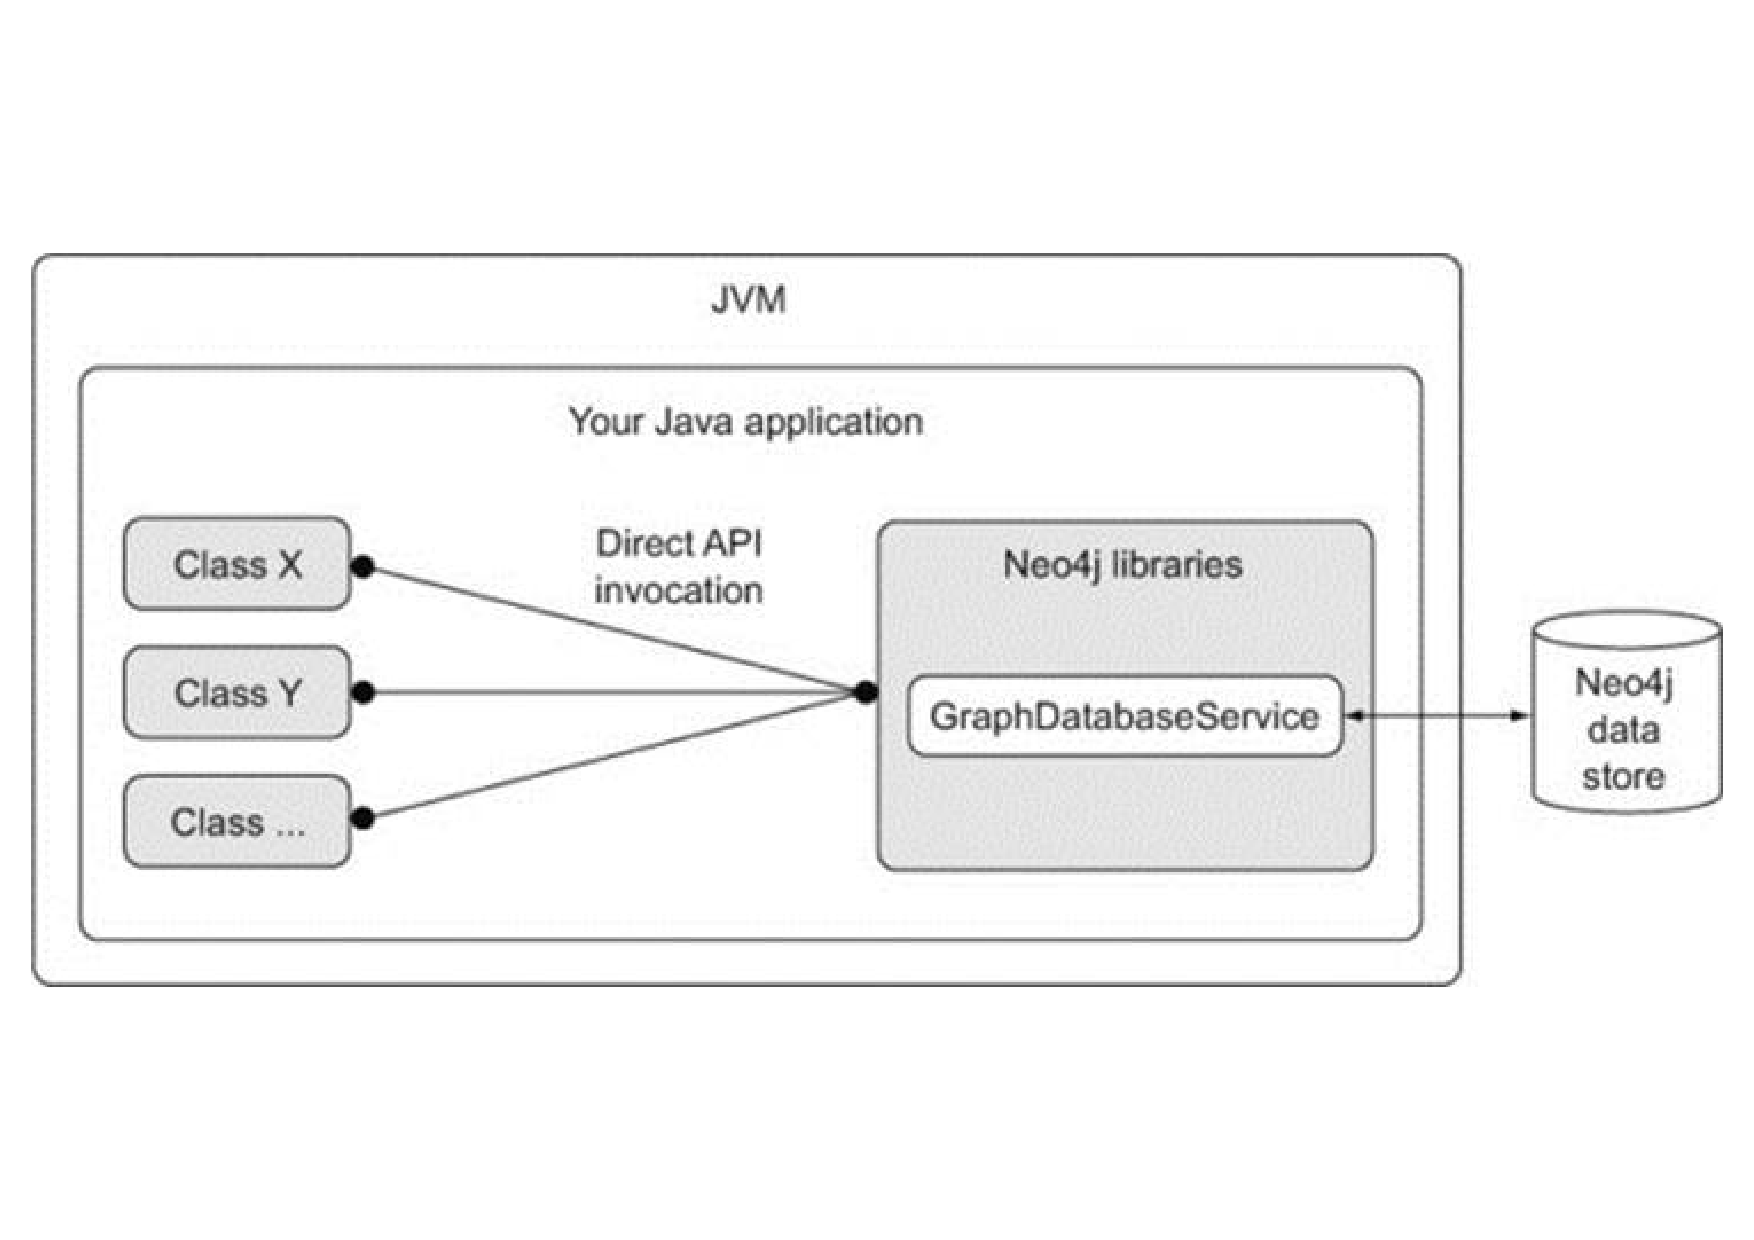
\includegraphics [width=12cm, height=10cm]{Figures/Embedded}
	\caption[Eingebettet]{Allgemeiner eingebetteteter Modus von Neo4j.}
	\label{fig:Embedded}
	\FloatBarrier
\end{figure}

\subsection{Der Server Modus}
Im Server Modus werden alle Anfragen von den Nutzern in einem eigenen Prozess verwaltet und mittels HTTP(Hypertext Transfer Protocol) als JSON-Formatiertes Dokument an die sogenannte REST API übermittelt \parencite{robinson2013graph}. Die REST API läuft in der Neo4j JVM und  verwaltet alle eintreffenden Anfragen der Nutzer und gibt diese an den GraphDatabaseService weiter, welcher die Bibliotheken verwaltet. \newline 
Der Server Modus ist für die Verwendung der High-Availability Fuktionen, welche das Nutzen der Datenbank auf mehren Systemen erlaubt, empfohlen\parencite{raj2015neo4j}. Da die Anfragen des Nutzer getrennt von der JVM der Neo4j Bibliotheken verwaltet werden und so mehrere Nutzer die Möglichkeit besitzen diese Funktionen zu Nutzen. Durch die  Übertragungsverzögerung innerhalb der Netzwerks und dem Übertragen durch eine weitere API ist der Geschwindigkeit langsamer als die des eingebetteten Modus. Dies wird in \ref{fig:Server} verdeutlicht.
\begin{figure}[!htb]
	\centering
	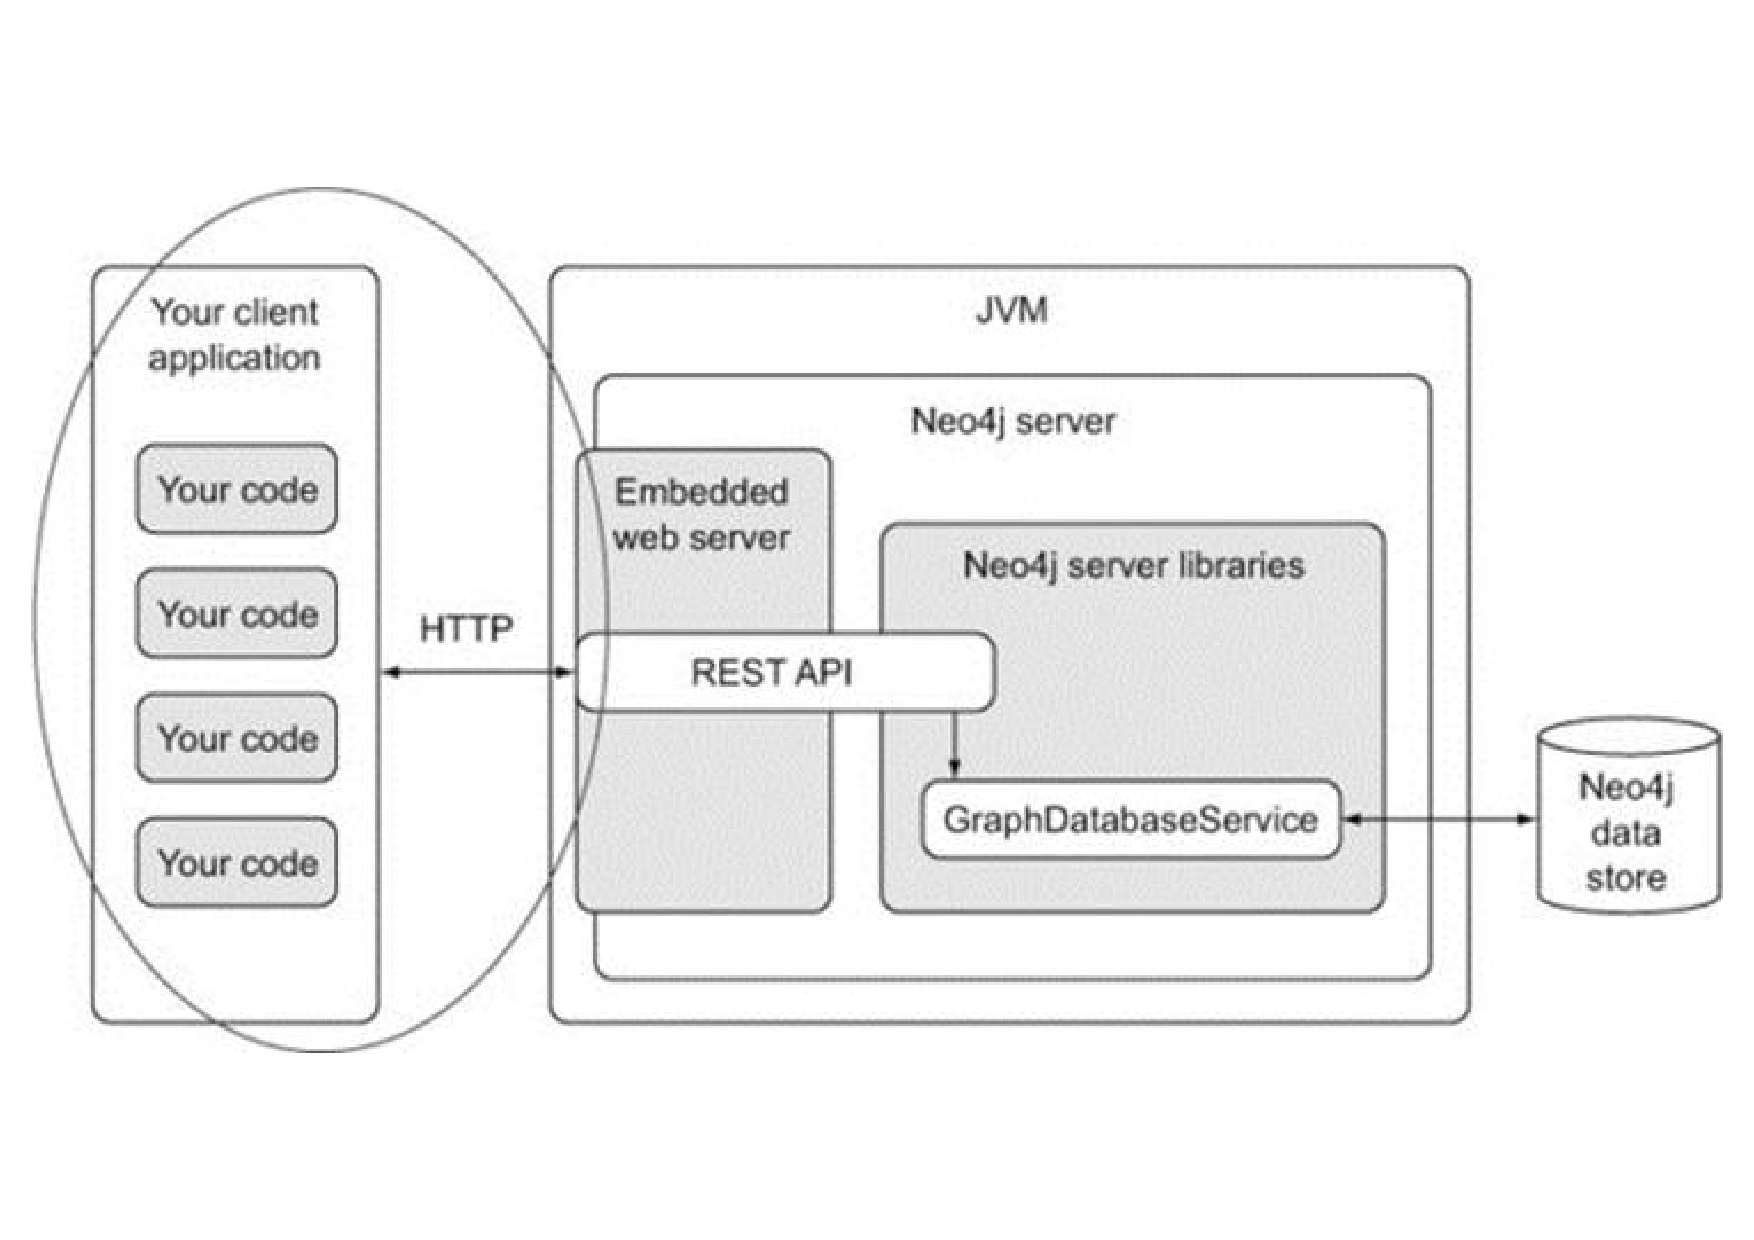
\includegraphics [width=14cm, height=12cm]{Figures/Server}
	\caption[Server]{Allgemeiner Servermodus von Neo4j.}
	\label{fig:Server}
	\FloatBarrier
\end{figure}

